% 【拆分生成】 answers.tex —— 2025 年·全国 2 卷 · 参考答案与详细解析片段
% 【拆分生成】 由 tools/split_project.py 自合并书 answers/2025_g2_sol.tex 包裹 answer 环境生成，勿手改
% 由 tools/md2tex.py 自 2025_数学真题_全国2_含解析.md 生成，勿手改（改源 MD 后重跑）


\begin{gknotice}
\textbf{解析归属}：本文档全部解析由编写者根据试题独立推导，\textbf{非官方标准答案}。推导过程均给出完整步骤以便核验；若与官方发布版本不一致，以官方为准。

\textbf{试题来源}：试题原文取自 deekur/gaokaomath（commit \texttt{34c13a6}，CC BY 4.0）之 \texttt{2025全国2} PDF。
\end{gknotice}

\par\medskip

\gkpart{一、单选题（每小题 5 分，共 40 分）}

\begin{answer}
\gksolhead{1}{}

\textbf{题目}　样本数据 $2,8,14,16,20$ 的平均数为（　　）

\begin{gkopts}(4)
\task A．$8$
\task B．$9$
\task C．$12$
\task D．$18$
\end{gkopts}

\textbf{解析}

平均数就是「总和除以个数」：
\[\bar x=\frac{2+8+14+16+20}{5}=\frac{60}{5}=12\]

\gkanswer{答案：C}

\begin{gktip}
\textbf{自检}：平均数必落在最小值 $2$ 与最大值 $20$ 之间，且这组数据「小的两个、大的三个」，均值偏向大数一侧，$12>\dfrac{2+20}{2}=11$ 。选项 A（$8$）是中位数 $14$ 与众数之类的干扰，D（$18$）明显偏大。
\end{gktip}

\par\medskip

\end{answer}
\begin{answer}
\gksolhead{2}{}

\textbf{题目}　已知 $z=1+\mathrm{i}$，则 $\dfrac{1}{z-1}=$（　　）

\begin{gkopts}(4)
\task A．$-\mathrm{i}$
\task B．$\mathrm{i}$
\task C．$-1$
\task D．$1$
\end{gkopts}

\textbf{解析}

先算分母：
\[z-1=(1+\mathrm{i})-1=\mathrm{i}\]

于是要算 $\dfrac1{\mathrm{i}}$。分子分母同乘 $\mathrm{i}$ 的共轭 $-\mathrm{i}$（或直接同乘 $\mathrm{i}$）：
\[\frac1{\mathrm{i}}=\frac{\mathrm{i}}{\mathrm{i}\cdot\mathrm{i}}=\frac{\mathrm{i}}{-1}=-\mathrm{i}\]

\gkanswer{答案：A}

\begin{gktip}
\textbf{值得记住的口诀}：$\dfrac1{\mathrm{i}}=-\mathrm{i}$。可用 $\mathrm{i}\cdot(-\mathrm{i})=-\mathrm{i}^2=1$ 一秒验证。
\end{gktip}

\par\medskip

\end{answer}
\begin{answer}
\gksolhead{3}{}

\textbf{题目}　已知集合 $A=\{-4,0,1,2,8\}$，$B=\left\{x\mid x^3=x\right\}$，则 $A\cap B=$（　　）

\begin{gkopts}(4)
\task A．$\{0,1,2\}$
\task B．$\{1,2,8\}$
\task C．$\{2,8\}$
\task D．$\{0,1\}$
\end{gkopts}

\textbf{解析}

\textbf{先把 $B$ 解出来}（这是本题唯一的计算量）：
\[x^3=x\ \Longrightarrow\ x^3-x=0\ \Longrightarrow\ x\left(x^2-1\right)=0\ \Longrightarrow\ x(x-1)(x+1)=0\]

\[B=\{-1,\ 0,\ 1\}\]

再取交集，逐个核对 $A$ 中元素是否在 $B$ 里：$-4$ ，$0$ ，$1$ ，$2$ ，$8$ 。

\[A\cap B=\{0,1\}\]

\gkanswer{答案：D}

\begin{gktip}
\textbf{易错点}：解方程时\textbf{两边同除以 $x$}，会丢掉根 $x=0$，得到 $B=\{-1,1\}$，进而误选出空集或其他答案。含 $x$ 的因式必须提出来，不能约掉。
\end{gktip}

\par\medskip

\end{answer}
\begin{answer}
\gksolhead{4}{}

\textbf{题目}　不等式 $\dfrac{x-4}{x-1}\ge 2$ 的解集是（　　）

\begin{gkopts}(2)
\task A．$\{x\mid -2\le x\le 1\}$
\task B．$\{x\mid x\le -2\}$
\task C．$\{x\mid -2\le x<1\}$
\task D．$\{x\mid x>1\}$
\end{gkopts}

\textbf{解析}

\textbf{绝不能直接两边乘 $(x-1)$}——它的符号未知。标准做法是\textbf{移项通分}：
\[\frac{x-4}{x-1}-2\ge 0\ \Longrightarrow\ \frac{(x-4)-2(x-1)}{x-1}\ge 0\ \Longrightarrow\ \frac{-x-2}{x-1}\ge 0\]

分子提负号（不等号方向翻转）：
\[\frac{x+2}{x-1}\le 0\]

分式 $\le 0$ 等价于「分子分母异号或分子为零」，且分母不为零：
\[(x+2)(x-1)\le 0\ \text{\text{且}}\ x\ne1\ \Longrightarrow\ -2\le x<1\]

\gkanswer{答案：C}

\begin{gktip}
\textbf{端点判定（本题的全部分差所在）}：
\begin{itemize}
\item $x=-2$：原式左边 $=\dfrac{-6}{-3}=2$，满足 $\ge2$，\textbf{取到} 
\item $x=1$：分母为零，\textbf{必须去掉} 
\end{itemize}

选项 A 恰恰是「把 $x=1$ 也算进去」的错误答案。凡分式不等式，写完解集第一件事就是回头排除使分母为零的点。
\end{gktip}

\par\medskip

\end{answer}
\begin{answer}
\gksolhead{5}{}

\textbf{题目}　在 $\triangle ABC$ 中，$BC=2$，$AC=1+\sqrt3$，$AB=\sqrt6$，则 $A=$（　　）

\begin{gkopts}(4)
\task A．$45^\circ$
\task B．$60^\circ$
\task C．$120^\circ$
\task D．$135^\circ$
\end{gkopts}

\textbf{解析}

\textbf{第一步，认清哪条边是 $A$ 的对边。} 角 $A$ 的对边是 $BC=2$，夹 $A$ 的两边是 $AB=\sqrt6$ 与 $AC=1+\sqrt3$。

\textbf{第二步，余弦定理}：
\[\cos A=\frac{AB^2+AC^2-BC^2}{2\cdot AB\cdot AC}\]

分子逐项算：$AB^2=6$，$AC^2=\left(1+\sqrt3\right)^2=1+2\sqrt3+3=4+2\sqrt3$，$BC^2=4$。
\[AB^2+AC^2-BC^2=6+\left(4+2\sqrt3\right)-4=6+2\sqrt3=2\sqrt3\left(\sqrt3+1\right)\]

（末一步把 $6=2\sqrt3\cdot\sqrt3$ 提出公因式 $2\sqrt3$，是本题化简的关键。）

分母：
\[2\cdot\sqrt6\cdot\left(1+\sqrt3\right)\]

相除时 $\left(1+\sqrt3\right)$ 整体约掉：
\[\cos A=\frac{2\sqrt3\left(\sqrt3+1\right)}{2\sqrt6\left(1+\sqrt3\right)}=\frac{\sqrt3}{\sqrt6}=\frac1{\sqrt2}=\frac{\sqrt2}{2}\]

又 $A\in(0^\circ,180^\circ)$，故
\[A=45^\circ\]

\gkanswer{答案：A}

\begin{gktip}
\textbf{数值自检}：$AC=1+\sqrt3\approx2.73$ 是最长边，故最大角是 $B$；$BC=2$ 是最短边，$A$ 应为最小角。$45^\circ$ 确实最小 （若误选 $120^\circ$ 或 $135^\circ$，最小边对最大角，立刻矛盾）。
\end{gktip}

\par\medskip

\end{answer}
\begin{answer}
\gksolhead{6}{}

\textbf{题目}　设抛物线 $C:y^2=2px\ (p>0)$ 的焦点为 $F$，点 $A$ 在 $C$ 上，过 $A$ 作 $C$ 的准线的垂线，垂足为 $B$．若直线 $BF$ 的方程为 $y=-2x+2$，则 $|AF|=$（　　）

\begin{gkopts}(4)
\task A．$3$
\task B．$4$
\task C．$5$
\task D．$6$
\end{gkopts}

\textbf{解析}

\textbf{第一步，用「$F$ 在直线 $BF$ 上」定出 $p$。}

抛物线 $y^2=2px$ 的焦点 $F\left(\dfrac p2,0\right)$，准线 $x=-\dfrac p2$。把 $F$ 代入 $y=-2x+2$：
\[0=-2\cdot\frac p2+2=-p+2\ \Longrightarrow\ p=2\]

于是
\[C:y^2=4x,\qquad F(1,0),\qquad \text{\text{准线} }x=-1\]

\textbf{第二步，求 $B$。} $B$ 在准线上，故 $x_B=-1$，代入直线：
\[y_B=-2\times(-1)+2=4\ \Longrightarrow\ B(-1,4)\]

\textbf{第三步，求 $A$。} $AB\perp$ 准线，而准线是竖直线，故 $AB$ 水平，$A$ 与 $B$ \textbf{纵坐标相同}：
\[y_A=4\ \Longrightarrow\ 16=4x_A\ \Longrightarrow\ x_A=4,\qquad A(4,4)\]

\textbf{第四步，用定义求 $|AF|$}（抛物线上的点到焦点距离 $=$ 到准线距离）：
\[|AF|=|AB|=x_A+\frac p2=4+1=5\]

\gkanswer{答案：C}

\begin{gktip}
\textbf{核对}：直接算距离 $|AF|=\sqrt{(4-1)^2+(4-0)^2}=\sqrt{9+16}=5$  与定义法一致。

\textbf{方法提醒}：凡出现「过抛物线上一点作准线的垂线」，第一反应就是\textbf{抛物线定义} $|AF|=|AB|$，可以绕开两点间距离公式。
\end{gktip}

\par\medskip

\end{answer}
\begin{answer}
\gksolhead{7}{}

\textbf{题目}　记 $S_n$ 为等差数列 $\{a_n\}$ 的前 $n$ 项和．若 $S_3=6$，$S_5=-5$，则 $S_6=$（　　）

\begin{gkopts}(4)
\task A．$-20$
\task B．$-15$
\task C．$-10$
\task D．$-5$
\end{gkopts}

\textbf{解析}

\textbf{最快的路：奇数项和 $=$ 项数 $\times$ 中间项。}

\[S_3=3a_2=6\ \Longrightarrow\ a_2=2,\qquad S_5=5a_3=-5\ \Longrightarrow\ a_3=-1\]

公差
\[d=a_3-a_2=-1-2=-3\]

于是 $a_1=a_2-d=2+3=5$，$a_4=a_3+d=-4$。

\[S_6=\frac{6\left(a_1+a_6\right)}{2}=3\left(a_3+a_4\right)=3\times(-1-4)=-15\]

（用了 $a_1+a_6=a_3+a_4$，等差数列中\textbf{下标和相等则项和相等}。）

\gkanswer{答案：B}

\begin{gktip}
\textbf{常规解法对照}（列方程组）：
\[S_3=3a_1+3d=6,\qquad S_5=5a_1+10d=-5\]
即 $a_1+d=2$、$a_1+2d=-1$，相减得 $d=-3$，$a_1=5$；
\[S_6=6a_1+15d=30-45=-15\ \]
\end{gktip}

\par\medskip

\end{answer}
\begin{answer}
\gksolhead{8}{}

\textbf{题目}　已知 $0<\alpha<\pi$，$\cos\dfrac{\alpha}{2}=\dfrac{\sqrt5}{5}$，则 $\sin\left(\alpha-\dfrac{\pi}{4}\right)=$（　　）

\begin{gkopts}(2)
\task A．$\dfrac{\sqrt2}{10}$
\task B．$\dfrac{\sqrt2}{5}$
\task C．$\dfrac{3\sqrt2}{10}$
\task D．$\dfrac{7\sqrt2}{10}$
\end{gkopts}

\textbf{解析}

\textbf{第一步，定半角的象限（必做，否则符号会错）。}

由 $0<\alpha<\pi$ 得 $0<\dfrac\alpha2<\dfrac\pi2$，故 $\sin\dfrac\alpha2>0$：
\[\sin\frac\alpha2=\sqrt{1-\cos^2\frac\alpha2}=\sqrt{1-\frac15}=\sqrt{\frac45}=\frac{2\sqrt5}{5}\]

\textbf{第二步，二倍角求 $\sin\alpha$、$\cos\alpha$。}
\[\sin\alpha=2\sin\frac\alpha2\cos\frac\alpha2=2\times\frac{2\sqrt5}{5}\times\frac{\sqrt5}{5}=2\times\frac{2\times5}{25}=\frac45\]
\[\cos\alpha=2\cos^2\frac\alpha2-1=2\times\frac15-1=-\frac35\]

\textbf{第三步，展开目标式。}
\[\sin\left(\alpha-\frac\pi4\right)=\sin\alpha\cos\frac\pi4-\cos\alpha\sin\frac\pi4=\frac{\sqrt2}{2}\left(\sin\alpha-\cos\alpha\right)\]

\[=\frac{\sqrt2}{2}\left(\frac45+\frac35\right)=\frac{\sqrt2}{2}\times\frac75=\frac{7\sqrt2}{10}\]

\gkanswer{答案：D}

\begin{gktip}
\textbf{自检}：$\cos\alpha=-\dfrac35<0$ 说明 $\alpha$ 是钝角，与 $\cos\dfrac\alpha2=\dfrac{\sqrt5}{5}\approx0.447\Rightarrow\dfrac\alpha2\approx63.4^\circ\Rightarrow\alpha\approx126.9^\circ$ 一致 

数值核对：$\sin\left(126.9^\circ-45^\circ\right)=\sin81.9^\circ\approx0.990$，而 $\dfrac{7\sqrt2}{10}\approx0.990$ 

\textbf{易错}：漏掉「$\dfrac\alpha2$ 在第一象限」的判断而给 $\sin\dfrac\alpha2$ 加负号；或把 $\cos\alpha$ 算成 $+\dfrac35$（选项 A 正是 $\dfrac{\sqrt2}{2}\times\dfrac15$，即 $\sin\alpha-\cos\alpha$ 算成 $\dfrac45-\dfrac35$ 的结果）。
\end{gktip}

\par\medskip

\end{answer}
\gkpart{二、多选题（每小题 6 分，共 18 分）}

\begin{answer}
\gksolhead{9}{}

\textbf{题目}　记 $S_n$ 为等比数列 $\{a_n\}$ 的前 $n$ 项和，$q$ 为 $\{a_n\}$ 的公比，$q>0$．若 $S_3=7$，$a_3=1$，则（　　）

\begin{gkopts}(4)
\task A．$q=\dfrac12$
\task B．$a_5=\dfrac19$
\task C．$S_5=8$
\task D．$a_n+S_n=8$
\end{gkopts}

\textbf{解析}

\textbf{第一步，先把 $q$ 解出来（后面四项全靠它）。}

由 $a_3=a_1q^2=1$ 得 $a_1=\dfrac1{q^2}$。代入 $S_3=a_1\left(1+q+q^2\right)=7$：
\[\frac{1+q+q^2}{q^2}=7\ \Longrightarrow\ 1+q+q^2=7q^2\ \Longrightarrow\ 6q^2-q-1=0\]

\[(3q+1)(2q-1)=0\ \Longrightarrow\ q=-\frac13\ \text{\text{或}}\ q=\frac12\]

由 $q>0$ 得
\[q=\frac12,\qquad a_1=\frac1{q^2}=4\]

于是通项与前 $n$ 项和为
\[a_n=4\left(\frac12\right)^{n-1}=2^{\,3-n},\qquad S_n=\frac{4\left[1-\left(\frac12\right)^n\right]}{1-\frac12}=8\left(1-2^{-n}\right)=8-2^{\,3-n}\]

（顺手核对：$S_3=8-2^0=7$ ，$a_3=2^0=1$ 。）

\par\medskip

\textbf{A 项}：$q=\dfrac12$，正是上面解出的值。 \textbf{A 正确}。

\textbf{B 项}：$a_5=2^{\,3-5}=2^{-2}=\dfrac14\ne\dfrac19$。 \textbf{B 错误}。

（$\dfrac19$ 是「误取 $q=-\dfrac13$ 分支」时会碰到的数字，属于典型干扰项。）

\textbf{C 项}：$S_5=8-2^{\,3-5}=8-\dfrac14=\dfrac{31}{4}=7.75\ne8$。 \textbf{C 错误}。

（$8$ 是 $n\to\infty$ 时的\textbf{无穷和} $\dfrac{a_1}{1-q}=\dfrac4{1/2}=8$，任何有限项和都\textbf{达不到} $8$。）

\textbf{D 项}：把通项与和式相加：
\[a_n+S_n=2^{\,3-n}+\left(8-2^{\,3-n}\right)=8\]

对一切 $n$ 恒成立。 \textbf{D 正确}。

\gkanswer{答案：AD}

\begin{gktip}
\textbf{结构洞察}：本题的漂亮之处在于 $S_n=8-a_n$——等比数列前 $n$ 项和「距离极限值的差」恰是当前项。C、D 两项互为镜像：$S_n$ 永远\textbf{差一个 $a_n$} 才到 $8$，所以 C 错而 D 对。
\end{gktip}

\par\medskip

\end{answer}
\begin{answer}
\gksolhead{10}{}

\textbf{题目}　已知 $f(x)$ 是定义在 $\mathbf{R}$ 上的奇函数，且当 $x>0$ 时，$f(x)=\left(x^2-3\right)\mathrm{e}^{x}+2$，则（　　）

\begin{gkopts}(1)
\task A．$f(0)=0$
\task B．当 $x<0$ 时，$f(x)=-\left(x^2-3\right)\mathrm{e}^{-x}-2$
\task C．$f(x)\ge 2$ 当且仅当 $x\ge\sqrt3$
\task D．$x=-1$ 是 $f(x)$ 的极大值点
\end{gkopts}

\textbf{解析}

\par\medskip

\textbf{A 项}：奇函数定义在 $\mathbf R$ 上，$0$ 在定义域内，取 $x=0$：
\[f(-0)=-f(0)\ \Longrightarrow\ f(0)=-f(0)\ \Longrightarrow\ f(0)=0\]

 \textbf{A 正确}。（注意「定义在 $\mathbf R$ 上」这个条件不可少——若 $0$ 不在定义域内则无此结论。）

\textbf{B 项}：设 $x<0$，则 $-x>0$，可用已知解析式：
\[f(-x)=\left[(-x)^2-3\right]\mathrm{e}^{-x}+2=\left(x^2-3\right)\mathrm{e}^{-x}+2\]

由奇性 $f(x)=-f(-x)$：
\[f(x)=-\left(x^2-3\right)\mathrm{e}^{-x}-2\]

与选项\textbf{逐字相同}。 \textbf{B 正确}。

\textbf{C 项}：先看 $x>0$ 的一半，此时
\[f(x)\ge2\iff\left(x^2-3\right)\mathrm{e}^{x}\ge0\iff x^2\ge3\iff x\ge\sqrt3\]

\textbf{这一半是对的，但「当且仅当」要求负半轴上不能有解}。检验一个具体点 $x=-1$：
\[f(-1)=-f(1)=-\left[\left(1-3\right)\mathrm{e}+2\right]=2\mathrm{e}-2\approx3.44\ \ge2\]

而 $-1<\sqrt3$，构成反例。 \textbf{C 错误}。

（更完整地：令 $t=-x>0$，$f(x)\ge2\iff\left(3-t^2\right)\mathrm{e}^{t}\ge4$。左端在 $t=0$ 处为 $3$、在 $t=1$ 处为 $2\mathrm{e}\approx5.44$、在 $t=\sqrt3$ 处为 $0$，故负半轴上的解集是一段区间，数值上约为 $x\in[-1.429,\,-0.323]$。）

\textbf{D 项}：先求 $x>0$ 时的导数：
\[f'(x)=2x\mathrm{e}^{x}+\left(x^2-3\right)\mathrm{e}^{x}=\left(x^2+2x-3\right)\mathrm{e}^{x}=(x+3)(x-1)\mathrm{e}^{x}\]

在 $(0,+\infty)$ 上 $(x+3)\mathrm{e}^x>0$，故 $f'$ 的符号由 $(x-1)$ 决定：$f$ 在 $(0,1)$ 递减、在 $(1,+\infty)$ 递增，$x=1$ 是\textbf{极小值点}。

\textbf{奇函数的导数是偶函数}：由 $f(-x)=-f(x)$ 两边求导得 $-f'(-x)=-f'(x)$，即
\[f'(-x)=f'(x)\]

于是 $f'(-1)=f'(1)=0$，且
\begin{itemize}
\item $x\in(-\infty,-1)$ 时 $-x>1$，$f'(x)=f'(-x)>0$，$f$ 递增；
\item $x\in(-1,0)$ 时 $0<-x<1$，$f'(x)=f'(-x)<0$，$f$ 递减。
\end{itemize}

左增右减，故 $x=-1$ 是\textbf{极大值点}。 \textbf{D 正确}。

\gkanswer{答案：ABD}

\begin{gktip}
\textbf{命题设计}：A、B 考奇函数的两个基本推论，D 考「奇函数把极小值点镜像成极大值点」，都是常规；真正的分水岭是 C——\textbf{它在正半轴上完全正确}，只要不去检查负半轴就会误判为真。凡看到「当且仅当」，必须\textbf{两个方向都验}，尤其是奇偶函数题里被忽略的另一半定义域。
\end{gktip}

\par\medskip

\end{answer}
\begin{answer}
\gksolhead{11}{}

\textbf{题目}　双曲线 $C:\dfrac{x^2}{a^2}-\dfrac{y^2}{b^2}=1\ (a>0,\ b>0)$ 的左、右焦点分别为 $F_1$，$F_2$，左、右顶点分别为 $A_1$，$A_2$，以 $F_1F_2$ 为直径的圆与 $C$ 的一条渐近线交于 $M$，$N$ 两点，且 $\angle NA_1M=\dfrac{5\pi}{6}$，则（　　）

\begin{gkopts}(1)
\task A．$\angle A_1MA_2=\dfrac{\pi}{6}$
\task B．$|MA_1|=2|MA_2|$
\task C．$C$ 的离心率为 $\sqrt{13}$
\task D．当 $a=\sqrt2$ 时，四边形 $NA_1MA_2$ 的面积为 $8\sqrt3$
\end{gkopts}

\textbf{解析}

\textbf{第一步（全题的钥匙）：求出 $M$、$N$ 的坐标。}

以 $F_1F_2$ 为直径的圆是 $x^2+y^2=c^2$；取渐近线 $y=\dfrac bax$，联立：
\[x^2+\frac{b^2}{a^2}x^2=c^2\ \Longrightarrow\ \frac{a^2+b^2}{a^2}x^2=c^2\ \Longrightarrow\ \frac{c^2}{a^2}x^2=c^2\ \Longrightarrow\ x=\pm a\]

\[M(a,\ b),\qquad N(-a,\ -b)\]

\textbf{这是双曲线的一条重要性质}：以焦距为直径的圆与渐近线的交点，横坐标恰是 $\pm a$、纵坐标恰是 $\pm b$（即该点在过顶点的竖直线上）。

\textbf{第二步，识别图形：$NA_1MA_2$ 是平行四边形。}

$M$ 与 $N$ 关于原点对称，$A_1(-a,0)$ 与 $A_2(a,0)$ 也关于原点对称，故对角线 $MN$ 与 $A_1A_2$ \textbf{互相平分}，四边形 $NA_1MA_2$ 是平行四边形。

\par\medskip

\textbf{A 项}：平行四边形的邻角互补：
\[\angle A_1MA_2=\pi-\angle NA_1M=\pi-\frac{5\pi}{6}=\frac\pi6\]

 \textbf{A 正确}。

\textbf{第三步，把角度条件翻译成 $a$、$b$ 的关系。}

$M(a,b)$ 与 $A_2(a,0)$ 横坐标相同，故 $MA_2\perp A_1A_2$，$\triangle MA_1A_2$ 是\textbf{直角三角形}（直角在 $A_2$），且 $\angle A_1MA_2=\dfrac\pi6$。于是
\[|MA_2|=b,\qquad |A_1A_2|=2a,\qquad \tan\frac\pi6=\frac{|A_1A_2|}{|MA_2|}=\frac{2a}{b}\]

\[\frac{1}{\sqrt3}=\frac{2a}{b}\ \Longrightarrow\ b=2\sqrt3\,a\ \Longrightarrow\ b^2=12a^2\]

\textbf{B 项}：在该直角三角形中，$\dfrac{|MA_1|}{|MA_2|}=\dfrac1{\cos\frac\pi6}=\dfrac{2}{\sqrt3}\approx1.155\ne2$。

具体地 $|MA_1|=\sqrt{(2a)^2+b^2}=\sqrt{4a^2+12a^2}=4a$，而 $|MA_2|=b=2\sqrt3a\approx3.46a$。 \textbf{B 错误}。

\textbf{C 项}：
\[c^2=a^2+b^2=a^2+12a^2=13a^2\ \Longrightarrow\ e=\frac ca=\sqrt{13}\]

 \textbf{C 正确}。

\textbf{D 项}：$a=\sqrt2$ 时 $b=2\sqrt3\times\sqrt2=2\sqrt6$。

平行四边形 $NA_1MA_2$ 的面积 $=2\times S_{\triangle MA_1A_2}$，而 $\triangle MA_1A_2$ 以 $A_1A_2$ 为底、以 $M$ 到 $x$ 轴的距离 $b$ 为高：
\[S=2\times\frac12\times|A_1A_2|\times b=2a\cdot b=2\sqrt2\times2\sqrt6=4\sqrt{12}=8\sqrt3\]

 \textbf{D 正确}。

\gkanswer{答案：ACD}

\begin{gktip}
\textbf{通用结论}（值得背）：此构型下平行四边形 $NA_1MA_2$ 的面积恒为 $2ab$。

\textbf{数值验算}：取 $a=\sqrt2$，则 $b=2\sqrt6\approx4.899$，$M\left(\sqrt2,\,4.899\right)$、$A_1\left(-\sqrt2,0\right)$、$N\left(-\sqrt2,-4.899\right)$。用向量算 $\angle NA_1M$：$\overrightarrow{A_1M}=(2\sqrt2,\,4.899)$，$\overrightarrow{A_1N}=(0,\,-4.899)$，夹角余弦 $=\dfrac{-24}{5.657\times4.899}=-0.866=\cos150^\circ$  与题设 $\dfrac{5\pi}{6}$ 吻合；面积 $=2\sqrt2\times2\sqrt6=8\sqrt3\approx13.86$ 。
\end{gktip}

\par\medskip

\end{answer}
\gkpart{三、填空题（每小题 5 分，共 15 分）}

\begin{answer}
\gksolhead{12}{}

\textbf{题目}　已知平面向量 $\boldsymbol{a}=(x,1)$，$\boldsymbol{b}=(x-1,2x)$，若 $\boldsymbol{a}\perp(\boldsymbol{a}-\boldsymbol{b})$，则 $|\boldsymbol{a}|=$ \gkblank{}．

\textbf{解析}

\textbf{先算差向量}（注意第一个分量的 $x$ 会抵消，这是本题的化简点）：
\[\boldsymbol{a}-\boldsymbol{b}=\big(x-(x-1),\ 1-2x\big)=(1,\ 1-2x)\]

\textbf{再用垂直 $\iff$ 数量积为零}：
\[\boldsymbol{a}\cdot(\boldsymbol{a}-\boldsymbol{b})=x\times1+1\times(1-2x)=x+1-2x=1-x=0\]

\[x=1\]

代回：$\boldsymbol{a}=(1,1)$，
\[|\boldsymbol{a}|=\sqrt{1^2+1^2}=\sqrt2\]

\gkanswer{答案：$\sqrt2$}

\begin{gktip}
\textbf{验算}：$x=1$ 时 $\boldsymbol b=(0,2)$，$\boldsymbol a-\boldsymbol b=(1,-1)$，$(1,1)\cdot(1,-1)=1-1=0$  确实垂直。

\textbf{易错}：把 $\boldsymbol a\perp(\boldsymbol a-\boldsymbol b)$ 误当成 $\boldsymbol a\perp\boldsymbol b$；或算完 $x$ 忘记回代求模，直接把 $x=1$ 当答案。
\end{gktip}

\par\medskip

\end{answer}
\begin{answer}
\gksolhead{13}{}

\textbf{题目}　若 $x=2$ 是函数 $f(x)=(x-1)(x-2)(x-a)$ 的极值点，则 $f(0)=$ \gkblank{}．

\textbf{解析}

\textbf{第一步，求导时用三项乘积的求导法则}（不必展开成三次多项式）：
\[f'(x)=(x-2)(x-a)+(x-1)(x-a)+(x-1)(x-2)\]

\textbf{第二步，代入 $x=2$——含因式 $(x-2)$ 的两项直接归零}：
\[f'(2)=\underbrace{0\cdot(2-a)}_{=0}+1\cdot(2-a)+\underbrace{1\cdot 0}_{=0}=2-a\]

$f$ 是多项式（处处可导），极值点必是驻点：
\[f'(2)=0\ \Longrightarrow\ a=2\]

\textbf{第三步，必须回头验证 $x=2$ 真是极值点}（驻点未必是极值点）。此时
\[f(x)=(x-1)(x-2)^2,\qquad f'(x)=(x-2)^2+2(x-1)(x-2)=(x-2)(3x-4)\]

$x$ 略小于 $2$ 时 $(x-2)<0$、$(3x-4)>0$，$f'<0$；$x$ 略大于 $2$ 时二者皆正，$f'>0$。\textbf{导数变号}，$x=2$ 确为极小值点 

\textbf{第四步，求值}：
\[f(0)=(0-1)(0-2)^2=(-1)\times4=-4\]

\gkanswer{答案：$-4$}

\begin{gktip}
\textbf{陷阱说明}：本题若 $a$ 取到使 $x=2$ 成为「二重驻点但不变号」的值，答案就会作废——所以第三步的变号检验不是走过场。这里恰好 $a=2$ 使 $(x-2)$ 成为二重因式，导数 $f'(x)=(x-2)(3x-4)$ 却只有一重 $(x-2)$，仍然变号，结论安全。
\end{gktip}

\par\medskip

\end{answer}
\begin{answer}
\gksolhead{14}{}

\textbf{题目}　一个底面半径为 $4\ \mathrm{cm}$，高为 $9\ \mathrm{cm}$ 的封闭圆柱形容器（容器壁厚度忽略不计）内有两个半径相等的铁球，则铁球半径的最大值为 \gkblank{} $\mathrm{cm}$．

\textbf{解析}

设球半径为 $r$，两球心为 $O_1$、$O_2$。约束有三条：

1. \textbf{不穿侧壁}：球心到圆柱轴的距离 $\le 4-r$；
2. \textbf{不穿上下底}：球心的高度 $z\in[r,\ 9-r]$；
3. \textbf{两球不重叠}：$|O_1O_2|\ge 2r$。

\textbf{关键一步：要让 $r$ 尽量大，就要让两球心尽量远。} 因此最优摆法是——一个球贴底、一个球贴顶，且二者在\textbf{轴截面的对角线方向}上分居两侧、各自紧贴侧壁。此时

\[\text{\text{竖直间距}}=9-2r,\qquad \text{\text{水平间距}}=2(4-r)=8-2r\]

代入条件 3：
\[(8-2r)^2+(9-2r)^2\ge(2r)^2\]

展开：
\[\left(64-32r+4r^2\right)+\left(81-36r+4r^2\right)\ge4r^2\]
\[4r^2-68r+145\ge0\]
\[(2r-5)(2r-29)\ge0\ \Longrightarrow\ r\le\frac52\ \text{\text{或}}\ r\ge\frac{29}{2}\]

$r\ge\dfrac{29}{2}=14.5$ 显然超出容器尺寸（还要求 $r\le4$），舍去。故
\[r_{\max}=\frac52\]

\textbf{取等验证}：$r=\dfrac52$ 时球心为 $\left(\dfrac32,0,\dfrac52\right)$ 与 $\left(-\dfrac32,0,\dfrac{13}{2}\right)$，
\[|O_1O_2|=\sqrt{3^2+4^2}=5=2r\ \]
到轴距离 $\dfrac32\le4-\dfrac52=\dfrac32$ （恰好贴壁），高度 $\dfrac52\ge r$、$\dfrac{13}2\le9-r$  全部满足。

\gkanswer{答案：$\dfrac52$}

\begin{gktip}
\textbf{轴截面视角（更快的写法）}：把问题压到过两球心的轴截面上，得到一个 $8\times9$ 的矩形内放两个半径 $r$ 的圆，两圆心分别为 $(r,r)$ 与 $(8-r,\,9-r)$，相切时圆心距为 $2r$：
\[(8-2r)^2+(9-2r)^2=4r^2\ \Longrightarrow\ r=\frac52\ \text{\text{或}}\ \frac{29}{2}\]
\textbf{注意勾股三元组}：$r=\dfrac52$ 时水平差 $3$、竖直差 $4$、圆心距 $5$，正是 $3\text-4\text-5$ 直角三角形——这是命题人埋的「整齐答案」信号。

\textbf{对照劣解}：两球上下叠放需 $4r\le9$ 即 $r\le2.25$；两球等高并排需 $2r\le2(4-r)$ 即 $r\le2$。都不如 $2.5$，可见「对角摆放」确实是最优。
\end{gktip}

\par\medskip

\end{answer}
\gkpart{四、解答题（共 77 分）}

\begin{answer}
\gksolhead{15}{13 分}

\textbf{题目}　已知函数 $f(x)=\cos(2x+\varphi)\ (0\le\varphi<\pi)$，$f(0)=\dfrac12$．

  (1) 求 $\varphi$；
  (2) 设函数 $g(x)=f(x)+f\left(x-\dfrac{\pi}{6}\right)$，求 $g(x)$ 的值域和单调区间．

\par\medskip

\textbf{(1) 解}

代入 $x=0$：
\[f(0)=\cos\varphi=\frac12\]

在区间 $[0,\pi)$ 内，$\cos\varphi=\dfrac12$ 只有一个解：
\[\varphi=\frac\pi3\]

（另一族解 $\varphi=-\dfrac\pi3+2k\pi$ 全部落在 $[0,\pi)$ 之外。）

\textbf{所以 $\varphi=\dfrac\pi3$。}

\par\medskip

\textbf{(2) 解}

\textbf{第一步，把 $g$ 化成「一个三角函数」。}

\[f(x)=\cos\left(2x+\frac\pi3\right),\qquad f\left(x-\frac\pi6\right)=\cos\left(2x-\frac\pi3+\frac\pi3\right)=\cos 2x\]

（\textbf{注意这里的巧合}：平移 $\dfrac\pi6$ 使 $2\times\dfrac\pi6=\dfrac\pi3$ 恰好抵消初相，第二项化成了最干净的 $\cos2x$。）

\[g(x)=\cos\left(2x+\frac\pi3\right)+\cos2x=\left(\frac12\cos2x-\frac{\sqrt3}{2}\sin2x\right)+\cos2x=\frac32\cos2x-\frac{\sqrt3}{2}\sin2x\]

辅助角合并，振幅
\[A=\sqrt{\left(\frac32\right)^2+\left(\frac{\sqrt3}{2}\right)^2}=\sqrt{\frac94+\frac34}=\sqrt3\]

\[g(x)=\sqrt3\left(\frac{\sqrt3}{2}\cos2x-\frac12\sin2x\right)=\sqrt3\cos\left(2x+\frac\pi6\right)\]

\textbf{校验}：$\sqrt3\cos\left(2x+\dfrac\pi6\right)=\sqrt3\left(\dfrac{\sqrt3}{2}\cos2x-\dfrac12\sin2x\right)=\dfrac32\cos2x-\dfrac{\sqrt3}{2}\sin2x$ 

\textbf{第二步，值域。} $\cos$ 的取值遍历 $[-1,1]$，故
\[\boxed{g(x)\text{ \text{的值域为}}\left[-\sqrt3,\ \sqrt3\right]}\]

\textbf{第三步，单调区间。} 令 $u=2x+\dfrac\pi6$，$u$ 关于 $x$ 单调递增，故 $g$ 的增减与 $\cos u$ 一致。

\textbf{递减}（$\cos u$ 在 $[2k\pi,\ 2k\pi+\pi]$ 递减）：
\[2k\pi\le 2x+\frac\pi6\le 2k\pi+\pi\ \Longrightarrow\ k\pi-\frac{\pi}{12}\le x\le k\pi+\frac{5\pi}{12}\]

\textbf{递增}（$\cos u$ 在 $[2k\pi-\pi,\ 2k\pi]$ 递增；等价地取 $[2k\pi+\pi,\ 2k\pi+2\pi]$）：
\[2k\pi+\pi\le 2x+\frac\pi6\le 2k\pi+2\pi\ \Longrightarrow\ k\pi+\frac{5\pi}{12}\le x\le k\pi+\frac{11\pi}{12}\]

\[\boxed{\text{\text{单调递减区间} }\left[k\pi-\frac{\pi}{12},\ k\pi+\frac{5\pi}{12}\right];\quad\text{\text{单调递增区间} }\left[k\pi+\frac{5\pi}{12},\ k\pi+\frac{11\pi}{12}\right],\ k\in\mathbf Z}\]

\begin{gktip}
\textbf{区间自检的三个要点}：
① 两类区间\textbf{首尾相接}（$k\pi+\dfrac{5\pi}{12}$ 既是减区间右端又是增区间左端），说明没有遗漏；
② 每个区间长度都是 $\dfrac\pi2$，等于周期 $T=\pi$ 的一半 ；
③ 取 $k=0$ 抽查：$g\left(-\dfrac\pi{12}\right)=\sqrt3\cos0=\sqrt3$（最大值），$g\left(\dfrac{5\pi}{12}\right)=\sqrt3\cos\pi=-\sqrt3$（最小值），中间确实从最高降到最低 
\end{gktip}

\par\medskip

\end{answer}
\begin{answer}
\gksolhead{16}{15 分}

\textbf{题目}　已知椭圆 $C:\dfrac{x^2}{a^2}+\dfrac{y^2}{b^2}=1\ (a>b>0)$ 的离心率为 $\dfrac{\sqrt2}{2}$，长轴长为 $4$．

  (1) 求 $C$ 的方程；
  (2) 过点 $(0,-2)$ 的直线 $l$ 与 $C$ 交于 $A$，$B$ 两点，$O$ 为坐标原点．若 $\triangle OAB$ 的面积为 $\sqrt2$，求 $|AB|$．

\par\medskip

\textbf{(1) 解}

长轴长 $=2a=4$，故 $a=2$。

由 $e=\dfrac ca=\dfrac{\sqrt2}{2}$ 得 $c=2\times\dfrac{\sqrt2}{2}=\sqrt2$。

\[b^2=a^2-c^2=4-2=2\]

\[\boxed{C:\ \frac{x^2}{4}+\frac{y^2}{2}=1}\]

\par\medskip

\textbf{(2) 解}

\textbf{第一步，排除斜率不存在的情形。} 若 $l:x=0$，则 $A$、$B$ 为 $\left(0,\pm\sqrt2\right)$，$O$、$A$、$B$ 三点共线，$\triangle OAB$ 不存在（面积为 $0\ne\sqrt2$），舍去。

故可设
\[l:\ y=kx-2\]

\textbf{第二步，联立并写出韦达定理。} 代入椭圆方程 $x^2+2y^2=4$：
\[x^2+2(kx-2)^2=4\ \Longrightarrow\ \left(1+2k^2\right)x^2-8kx+4=0\]

设 $A(x_1,y_1)$、$B(x_2,y_2)$，则
\[x_1+x_2=\frac{8k}{1+2k^2},\qquad x_1x_2=\frac{4}{1+2k^2}\]

有两个交点要求
\[\Delta=64k^2-16\left(1+2k^2\right)=32k^2-16>0\ \Longrightarrow\ k^2>\frac12\]

\textbf{第三步（本题最省力的一步）：把面积化成 $|x_1-x_2|$。}

用坐标形式的面积公式（$O$ 为原点）：
\[S_{\triangle OAB}=\frac12\left|x_1y_2-x_2y_1\right|=\frac12\left|x_1\left(kx_2-2\right)-x_2\left(kx_1-2\right)\right|=\frac12\left|-2x_1+2x_2\right|=\left|x_1-x_2\right|\]

（$kx_1x_2$ 项互相抵消——这正是「直线过 $y$ 轴上的定点 $(0,-2)$、而 $|OP|=2$」带来的便利：$S=\dfrac12\cdot|OP|\cdot\left|x_1-x_2\right|=\left|x_1-x_2\right|$。）

\textbf{第四步，解方程。} 由 $S=\sqrt2$ 得 $\left|x_1-x_2\right|=\sqrt2$，即
\[\left(x_1-x_2\right)^2=\left(x_1+x_2\right)^2-4x_1x_2=\frac{64k^2}{\left(1+2k^2\right)^2}-\frac{16}{1+2k^2}=\frac{32k^2-16}{\left(1+2k^2\right)^2}=2\]

\[32k^2-16=2\left(1+2k^2\right)^2=2\left(4k^4+4k^2+1\right)=8k^4+8k^2+2\]

\[8k^4-24k^2+18=0\ \Longrightarrow\ 4k^4-12k^2+9=0\ \Longrightarrow\ \left(2k^2-3\right)^2=0\]

\[k^2=\frac32\]

\textbf{（完全平方！）} 说明满足条件的直线只有 $k=\pm\dfrac{\sqrt6}{2}$ 两条，且 $k^2=\dfrac32>\dfrac12$ 满足判别式条件 

\textbf{第五步，求 $|AB|$。} 此时 $1+2k^2=4$，
\[\left|x_1-x_2\right|=\sqrt2,\qquad |AB|=\sqrt{1+k^2}\cdot\left|x_1-x_2\right|=\sqrt{1+\frac32}\times\sqrt2=\sqrt{\frac52}\times\sqrt2=\sqrt5\]

\[\boxed{|AB|=\sqrt5}\]

\begin{gktip}
\textbf{数值验算}（取 $k=\sqrt{1.5}$）：方程为 $4x^2-8\sqrt{1.5}\,x+4=0$，即 $x^2-2\sqrt{1.5}\,x+1=0$，两根 $x=\sqrt{1.5}\pm\sqrt{0.5}$，
\[x_1\approx1.9319,\quad x_2\approx0.5176,\quad \left|x_1-x_2\right|\approx1.4142=\sqrt2\ \]
对应 $y_1\approx0.3660$、$y_2\approx-1.3660$，代入椭圆：$\dfrac{1.9319^2}{4}+\dfrac{0.3660^2}{2}=0.9330+0.0670=1$ 
\[|AB|=\sqrt{1.4142^2+1.7321^2}=\sqrt{2+3}=\sqrt5\approx2.2361\ ,\qquad S=\left|x_1-x_2\right|=\sqrt2\ \]
\end{gktip}

\par\medskip

\end{answer}
\begin{answer}
\gksolhead{17}{15 分}

\textbf{题目}　如图，在四边形 $ABCD$ 中，$AB\parallel CD$，$\angle DAB=90^\circ$，$F$ 为 $CD$ 的中点，点 $E$ 在 $AB$ 上，$EF\parallel AD$，$AB=3AD$，$CD=2AD$．将四边形 $EFDA$ 沿 $EF$ 翻折至四边形 $EFD'A'$，使得面 $EFD'A'$ 与面 $EFCB$ 所成的二面角为 $60^\circ$．

\begin{center}% 2025 全国 2 卷 17：正方形沿 EF 翻折后的四棱锥体（A、D 翻折到 A'、D'）
% 立体坐标 E(0,0,0)、B(2,0,0)、F(0,1,0)、C(1,1,0)、A'(1/2,0,√3/2)、D'(1/2,1,√3/2)，
% 翻折前的位置 A(-1,0,0)、D(-1,1,0) 以虚影正方形 AEFD 保留，示折痕 EF 的来源。
% 画布投影：(x,y,z) -> x·(1,0) + y·(0.35,0.45) + z·(0,1)。
% 虚线：被遮挡的 EF、FC、CB、FD'、D'C，以及翻折前的虚影边 AE、AD、DF。
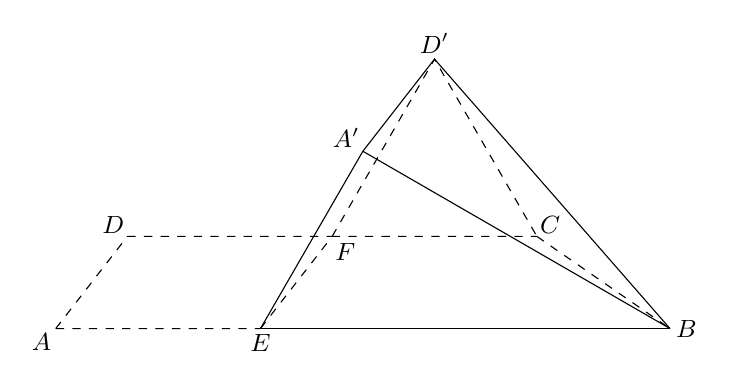
\begin{tikzpicture}[scale=2.6, font=\small]
  \coordinate (E)  at (0,0);
  \coordinate (B)  at (2,0);
  \coordinate (F)  at (0.35,0.45);
  \coordinate (C)  at (1.35,0.45);
  \coordinate (Ap) at (0.5,0.866);
  \coordinate (Dp) at (0.85,1.316);
  \coordinate (A)  at (-1,0);
  \coordinate (D)  at (-0.65,0.45);
  % 可见实线
  \draw (E) -- (B);
  \draw (E) -- (Ap) -- (Dp) -- (B);
  \draw (Ap) -- (B);
  \draw[dashed] (C) -- (B);
  % 被遮挡
  \draw[dashed] (E) -- (F) -- (C);
  \draw[dashed] (F) -- (Dp) -- (C);
  % 翻折前的虚影正方形 AEFD
  \draw[dashed] (A) -- (E)  (A) -- (D)  (D) -- (F);
  \node[below left,  inner sep=1.5pt] at (A)  {$A$};
  \node[above left,  inner sep=1pt]   at (D)  {$D$};
  \node[below,       inner sep=2pt]   at (E)  {$E$};
  \node[below right, inner sep=1pt, yshift=-1.5pt] at (F) {$F$};
  \node[above right, inner sep=1pt]   at (C)  {$C$};
  \node[right,       inner sep=2pt]   at (B)  {$B$};
  \node[above left,  inner sep=1pt]   at (Ap) {$A'$};
  \node[above,       inner sep=2pt]   at (Dp) {$D'$};
\end{tikzpicture}
\end{center}

  (1) 证明：$A'B\parallel$ 平面 $CD'F$；
  (2) 求面 $BCD'$ 与面 $EFD'A'$ 所成的二面角的正弦值．

\par\medskip

\textbf{准备：先把翻折前的平面图形量清楚（这一步做不对，后面全错）。}

设 $AD=1$，则 $AB=3$、$CD=2$。在原平面图形中以 $A$ 为原点、$AB$ 为横轴、$AD$ 为纵轴：
\[A(0,0),\quad B(3,0),\quad D(0,1),\quad C(2,1)\]

（$AB\parallel CD$ 且 $\angle DAB=90^\circ$ $\Rightarrow$ $AD\perp AB$ 且 $AD\perp CD$，故 $ABCD$ 是直角梯形，$C$ 与 $D$ 等高。）

\begin{itemize}
\item $F$ 是 $CD$ 中点：$F(1,1)$，且 $DF=FC=1$；
\item $E$ 在 $AB$ 上且 $EF\parallel AD$（竖直）：$E(1,0)$，$AE=1$、$EB=2$。
\end{itemize}

于是折痕两侧分别是：

\begin{itemize}
\item \textbf{四边形 $EFDA$：边长为 $1$ 的正方形}（$EA=AD=DF=FE=1$，四角皆直角）；
\item \textbf{四边形 $EFCB$：直角梯形}（$EF=1$、$FC=1$、$EB=2$，且 $EF\perp EB$、$EF\perp FC$）。
\end{itemize}

\textbf{两条贯穿全题的垂直关系}（翻折不改变半平面内部的角度）：
\[EF\perp EA'\ \text{\text{且}}\ EF\perp EB;\qquad EF\perp FD'\ \text{\text{且}}\ EF\perp FC\]

因此 $\angle A'EB$ 就是二面角 $A'\text-EF\text-B$ 的平面角：
\[\angle A'EB=60^\circ\]

\par\medskip

\textbf{(1) 证明}

\textbf{综合法（不用坐标，三行结束）}：

由上，$EA'\cap EB=E$ 且 $EA',EB\subset$ 平面 $A'EB$，又 $EF\perp EA'$、$EF\perp EB$，故
\[EF\perp\text{\text{平面} }A'EB\]

同理 $FD'\cap FC=F$，$EF\perp FD'$、$EF\perp FC$，故
\[EF\perp\text{\text{平面} }CD'F\]

\textbf{两个平面同垂直于直线 $EF$，因此互相平行}：
\[\text{\text{平面} }A'EB\ \parallel\ \text{\text{平面} }CD'F\]

而 $A'B\subset$ 平面 $A'EB$，且 $A'B\not\subset$ 平面 $CD'F$，由「面面平行 $\Rightarrow$ 其中一面内的任一直线平行于另一面」得
\[A'B\parallel\text{\text{平面} }CD'F\qquad\blacksquare\]

\par\medskip

\textbf{(2) 解}

\textbf{建系}：以 $E$ 为原点，$EB$ 方向为 $x$ 轴、$EF$ 方向为 $y$ 轴、过 $E$ 且垂直于底面 $EFCB$ 的方向为 $z$ 轴。

底面上三点直接读出（$EB=2$，$FC=1$ 且 $FC\parallel EB$）：
\[E(0,0,0),\quad F(0,1,0),\quad B(2,0,0),\quad C(1,1,0)\]

$A'$ 在 $xOz$ 平面内，$|EA'|=1$ 且与 $x$ 轴正向成 $60^\circ$：
\[A'\left(\cos60^\circ,\ 0,\ \sin60^\circ\right)=\left(\frac12,\ 0,\ \frac{\sqrt3}{2}\right)\]

由 $A'EFD'$ 仍是正方形，$\overrightarrow{FD'}=\overrightarrow{EA'}$：
\[D'=F+\overrightarrow{EA'}=\left(\frac12,\ 1,\ \frac{\sqrt3}{2}\right)\]

\textbf{（顺带把 (1) 再验一遍）}：$C$、$D'$、$F$ 三点的 $y$ 坐标全为 $1$，即平面 $CD'F$ 就是平面 $y=1$；$\overrightarrow{A'B}=\left(\dfrac32,0,-\dfrac{\sqrt3}{2}\right)$ 的 $y$ 分量为 $0$，与法向量 $(0,1,0)$ 垂直，且 $A'$ 的 $y$ 坐标为 $0\ne1$ 

\textbf{求平面 $EFD'A'$ 的法向量 $\boldsymbol n_1$}：该平面含 $\overrightarrow{EF}=(0,1,0)$ 与 $\overrightarrow{EA'}=\left(\dfrac12,0,\dfrac{\sqrt3}{2}\right)$，
\[\boldsymbol n_1=\overrightarrow{EF}\times\overrightarrow{EA'}=\left(\frac{\sqrt3}{2},\ 0,\ -\frac12\right)\ \parallel\ \left(\sqrt3,\ 0,\ -1\right)\]

\textbf{求平面 $BCD'$ 的法向量 $\boldsymbol n_2$}：
\[\overrightarrow{BC}=(-1,1,0),\qquad \overrightarrow{BD'}=\left(-\frac32,\ 1,\ \frac{\sqrt3}{2}\right)\]
\[\boldsymbol n_2=\overrightarrow{BC}\times\overrightarrow{BD'}=\left(\frac{\sqrt3}{2},\ \frac{\sqrt3}{2},\ \frac12\right)\ \parallel\ \left(\sqrt3,\ \sqrt3,\ 1\right)\]

\textbf{求夹角}：
\[\cos\theta=\frac{\left|\boldsymbol n_1\cdot\boldsymbol n_2\right|}{\left|\boldsymbol n_1\right|\left|\boldsymbol n_2\right|}=\frac{\left|\sqrt3\times\sqrt3+0\times\sqrt3+(-1)\times1\right|}{\sqrt{3+0+1}\cdot\sqrt{3+3+1}}=\frac{|3-1|}{2\sqrt7}=\frac{1}{\sqrt7}=\frac{\sqrt7}{7}\]

\[\sin\theta=\sqrt{1-\frac17}=\sqrt{\frac67}=\frac{\sqrt{42}}{7}\]

\[\boxed{\text{\text{所求二面角的正弦值为}}\frac{\sqrt{42}}{7}}\]

\begin{gktip}
\textbf{数值核对}：$\dfrac{\sqrt{42}}{7}\approx0.9258$，对应角度约 $67.79^\circ$；$\cos\theta=\dfrac{\sqrt7}{7}\approx0.3780$  二者平方和为 $1$。

\textbf{建系合理性检查}：$|EA'|=\sqrt{\dfrac14+\dfrac34}=1$ ，$|FD'|=1$ ，$\overrightarrow{EF}\cdot\overrightarrow{EA'}=0$ （正方形的直角保住了），$A'$ 与 $x$ 轴正向夹角 $=60^\circ$ （二面角条件）。

\textbf{易错}：题目问的是\textbf{正弦值}，法向量夹角算出来的是余弦，务必再开方转换一次；另外二面角可能是钝角，但正弦值不受影响（$\sin\theta=\sin(\pi-\theta)$），故取绝对值不影响答案。
\end{gktip}

\par\medskip

\end{answer}
\begin{answer}
\gksolhead{18}{17 分}

\textbf{题目}　已知函数 $f(x)=\ln(1+x)-x+\dfrac12x^2-kx^3$，其中 $0<k<\dfrac13$．

  (1) 证明：$f(x)$ 在区间 $(0,+\infty)$ 存在唯一的极值点和唯一的零点；
  (2) 设 $x_1$，$x_2$ 分别为 $f(x)$ 在区间 $(0,+\infty)$ 的极值点和零点．
  　① 设函数 $g(t)=f(x_1+t)-f(x_1-t)$．证明：$g(t)$ 在区间 $(0,x_1)$ 单调递减；
  　② 比较 $2x_1$ 与 $x_2$ 的大小，并证明你的结论．

\par\medskip

\textbf{(1) 证明}

\textbf{第一步，求导并作出全题的关键化简。}

定义域为 $(-1,+\infty)$。
\[f'(x)=\frac1{1+x}-1+x-3kx^2\]

先合并前两项：$\dfrac1{1+x}-1=\dfrac{-x}{1+x}$，于是
\[f'(x)=-\frac{x}{1+x}+x-3kx^2=x\left(1-\frac1{1+x}\right)-3kx^2=x\cdot\frac{x}{1+x}-3kx^2\]

\[\boxed{f'(x)=x^2\left(\frac1{1+x}-3k\right)}\]

\textbf{这个因式分解出 $x^2$ 是全题的枢纽}：在 $(0,+\infty)$ 上 $x^2>0$，导数符号完全由括号决定。

\textbf{第二步，极值点的存在唯一性。}

记 $\varphi(x)=\dfrac1{1+x}-3k$。在 $(0,+\infty)$ 上 $\varphi$ \textbf{严格递减}，且
\[\varphi(0)=1-3k>0\quad(\text{\text{因} }k<\tfrac13),\qquad \varphi(x)\xrightarrow[x\to+\infty]{}-3k<0\]

故 $\varphi$ 在 $(0,+\infty)$ 上有唯一零点，解出即
\[x_1=\frac{1}{3k}-1>0\qquad\left(\text{\text{因} }0<3k<1\right)\]

于是 $f$ 在 $(0,x_1)$ 上 $f'>0$（递增）、在 $(x_1,+\infty)$ 上 $f'<0$（递减），$x_1$ 是\textbf{唯一的极值点（极大值点）} 

\textbf{第三步，零点的存在唯一性。}

注意
\[f(0)=\ln1-0+0-0=0\]

\begin{itemize}
\item 在 $(0,x_1]$ 上 $f$ \textbf{严格递增}，故 $f(x)>f(0)=0$，\textbf{没有零点}（且顺带得到 $f(x_1)>0$）；
\item 在 $[x_1,+\infty)$ 上 $f$ \textbf{严格递减}，至多一个零点。为说明确实存在，用经典不等式 $\ln(1+x)\le x$（$x>-1$）：
\end{itemize}
\[f(x)\le x-x+\frac12x^2-kx^3=x^2\left(\frac12-kx\right)\]

取 $x_0=\dfrac1k$（此时 $\dfrac12-kx_0=-\dfrac12<0$）：
\[f\left(\frac1k\right)\le\frac1{k^2}\times\left(-\frac12\right)<0\]

而 $x_0=\dfrac1k>\dfrac1{3k}>x_1$，故 $x_0$ 落在递减区间内。由零点存在定理，$f$ 在 $\left(x_1,\dfrac1k\right)$ 内有零点；结合严格单调，该零点唯一。

综上，$f$ 在 $(0,+\infty)$ 上\textbf{恰有一个极值点 $x_1$ 与一个零点 $x_2$，且 $x_2>x_1$} $\blacksquare$

\par\medskip

\textbf{(2)① 证明}

\textbf{关键改写}：由 $x_1=\dfrac1{3k}-1$ 得 $3k=\dfrac1{1+x_1}$，代回导数式：
\[f'(x)=x^2\left(\frac1{1+x}-\frac1{1+x_1}\right)=\frac{x^2\left(x_1-x\right)}{(1+x)\left(1+x_1\right)}\]

\textbf{求 $g'$（注意第二项的链式法则会带出负号，两项因此同号相加）}：
\[g'(t)=f'\left(x_1+t\right)\cdot 1-f'\left(x_1-t\right)\cdot(-1)=f'\left(x_1+t\right)+f'\left(x_1-t\right)\]

逐项代入（$x_1-\left(x_1+t\right)=-t$，$x_1-\left(x_1-t\right)=t$）：
\[g'(t)=\frac{\left(x_1+t\right)^2(-t)}{\left(1+x_1+t\right)\left(1+x_1\right)}+\frac{\left(x_1-t\right)^2\cdot t}{\left(1+x_1-t\right)\left(1+x_1\right)}\]

\[=\frac{t}{1+x_1}\left[\frac{\left(x_1-t\right)^2}{1+x_1-t}-\frac{\left(x_1+t\right)^2}{1+x_1+t}\right]\]

\textbf{构造辅助函数比较方括号内两项}。令
\[h(u)=\frac{u^2}{1+u}\qquad(u>0)\]

\[h'(u)=\frac{2u(1+u)-u^2}{(1+u)^2}=\frac{u^2+2u}{(1+u)^2}=\frac{u(u+2)}{(1+u)^2}>0\]

故 $h$ 在 $(0,+\infty)$ 上\textbf{严格递增}。

对 $t\in\left(0,x_1\right)$ 有 $0<x_1-t<x_1+t$，于是
\[h\left(x_1-t\right)<h\left(x_1+t\right)\ \Longrightarrow\ \left[\ \cdots\ \right]<0\]

又 $\dfrac{t}{1+x_1}>0$，所以
\[g'(t)<0\qquad\text{\text{对一切} }t\in\left(0,x_1\right)\]

故 $g(t)$ 在区间 $\left(0,x_1\right)$ 上\textbf{单调递减} $\blacksquare$

\begin{gktip}
\textbf{本问的设计意图}：$g(t)=f\left(x_1+t\right)-f\left(x_1-t\right)$ 度量的是 $f$ 的图象\textbf{关于极值点 $x_1$ 的左右不对称程度}。$g$ 递减且 $g(0)=0$，意味着「往右走掉得比往左走掉得快」——这正是第 ② 问的全部内容。
\end{gktip}

\par\medskip

\textbf{(2)② 解}

\textbf{结论：$2x_1>x_2$。}

\textbf{证明}：$g$ 在闭区间 $\left[0,x_1\right]$ 上连续（因 $x_1-t\in\left[0,x_1\right]$ 始终在 $f$ 的定义域 $(-1,+\infty)$ 内），在 $\left(0,x_1\right)$ 内严格递减，且
\[g(0)=f\left(x_1\right)-f\left(x_1\right)=0\]

故
\[g\left(x_1\right)<g(0)=0\]

而由定义
\[g\left(x_1\right)=f\left(2x_1\right)-f(0)=f\left(2x_1\right)-0=f\left(2x_1\right)\]

（用到 (1) 中算出的 $f(0)=0$。）所以
\[f\left(2x_1\right)<0=f\left(x_2\right)\]

\textbf{最后一步，用单调性把函数值的大小翻译成自变量的大小}：$2x_1>x_1$ 且 $x_2>x_1$，两点都落在 $f$ 的\textbf{严格递减}区间 $\left(x_1,+\infty\right)$ 内，函数值小的自变量必然更大，故
\[\boxed{2x_1>x_2}\]

$\blacksquare$

\begin{gktip}
\textbf{数值验算}（取 $k=0.2$，满足 $0<k<\dfrac13$）：
\[x_1=\frac1{0.6}-1=\frac23\approx0.6667,\qquad 2x_1\approx1.3333\]
数值求根得 $x_2\approx0.9168$，确有 $2x_1>x_2$ 
且 $f\left(2x_1\right)=\ln 2.3333-1.3333+\dfrac{1.3333^2}{2}-0.2\times1.3333^3\approx-0.0712<0$ 

再取 $k=0.3$：$x_1=\dfrac1{0.9}-1\approx0.1111$，$2x_1\approx0.2222$，$x_2\approx0.1492<0.2222$ 
再取 $k=0.01$：$x_1\approx32.33$，$2x_1\approx64.67$，$x_2\approx24.6$ 之后（$f\left(2x_1\right)\approx-674<0$）

\textbf{方法总结}：这是一道「不动点 $\to$ 对称化 $\to$ 单调性比较」的三级递进题。第 (2)① 问看似突兀的 $g(t)$，其实就是\textbf{把 $x_2$ 与 $2x_1$ 的比较问题，转化成对 $f\left(2x_1\right)$ 符号的判断}——而 $f\left(2x_1\right)$ 的符号又恰好是 $g$ 在端点 $t=x_1$ 处的值。凡遇到「比较 $2x_1$ 与 $x_2$」这类题，标准套路就是构造 $f\left(x_1+t\right)-f\left(x_1-t\right)$。
\end{gktip}

\par\medskip

\end{answer}
\begin{answer}
\gksolhead{19}{17 分}

\textbf{题目}　甲、乙两人进行乒乓球练习，每个球胜者得 $1$ 分，负者得 $0$ 分．设每个球甲胜的概率为 $p\ \left(\dfrac12<p<1\right)$，乙胜的概率为 $q$，$p+q=1$，且各球的胜负相互独立．对正整数 $k\ge 2$，记 $p_k$ 为打完 $k$ 个球后甲比乙至少多得 $2$ 分的概率，$q_k$ 为打完 $k$ 个球后乙比甲至少多得 $2$ 分的概率．

  (1) 求 $p_3$，$p_4$（用 $p$ 表示）；
  (2) 若 $\dfrac{p_4-p_3}{q_4-q_3}=4$，求 $p$；
  (3) 证明：对任意正整数 $m$，$p_{2m+1}-q_{2m+1}<p_{2m}-q_{2m}<p_{2m+2}-q_{2m+2}$．

\par\medskip

\textbf{统一记号（贯穿三问）}

设打完 $k$ 个球后甲得 $X$ 分，则 $X\sim B(k,p)$，乙得 $k-X$ 分，\textbf{分差}
\[S_k=X-(k-X)=2X-k\]

于是
\[p_k=P\left(S_k\ge2\right),\qquad q_k=P\left(S_k\le-2\right)\]

\textbf{关键的奇偶性}：$S_k=2X-k$ 与 $k$ \textbf{同奇偶}。$k$ 为偶数时 $S_k$ 取偶数值，$k$ 为奇数时 $S_k$ 取奇数值——这一点是第 (3) 问的立足点。

\par\medskip

\textbf{(1) 解}

\textbf{求 $p_3$}：$S_3=2X-3\ge2\iff X\ge2.5$，而 $X$ 是整数且 $X\le3$，故只有 $X=3$（甲三球全胜）：
\[p_3=p^3\]

\textbf{求 $p_4$}：$S_4=2X-4\ge2\iff X\ge3$，即 $X=3$ 或 $X=4$：
\[p_4=\binom43p^3q+p^4=4p^3(1-p)+p^4=4p^3-4p^4+p^4\]

\[\boxed{p_3=p^3,\qquad p_4=4p^3-3p^4=p^3(4-3p)}\]

\textbf{校验}：$p=1$ 时 $p_3=1$、$p_4=4-3=1$ （甲必胜则必定领先 $2$ 分以上）；$p=\dfrac12$ 时 $p_4=\dfrac18\times\dfrac52=\dfrac5{16}$，而直接数：$X\ge3$ 的概率 $=\dfrac{\binom43+\binom44}{16}=\dfrac{5}{16}$ 

\par\medskip

\textbf{(2) 解}

\textbf{利用对称性}：把甲乙互换，$p\leftrightarrow q$，则 $p_k$ 与 $q_k$ 互换。故由 (1) 直接得
\[q_3=q^3,\qquad q_4=4q^3-3q^4\]

\textbf{分别作差（都能提出漂亮的公因式）}：
\[p_4-p_3=\left(4p^3-3p^4\right)-p^3=3p^3-3p^4=3p^3(1-p)=3p^3q\]
\[q_4-q_3=3q^3(1-q)=3q^3p\]

\textbf{相除}：
\[\frac{p_4-p_3}{q_4-q_3}=\frac{3p^3q}{3q^3p}=\frac{p^2}{q^2}=\left(\frac pq\right)^2\]

由题设等于 $4$，又 $p,q>0$，故
\[\frac pq=2\ \Longrightarrow\ p=2q=2(1-p)\ \Longrightarrow\ 3p=2\]

\[\boxed{p=\frac23}\]

\textbf{检验}：$\dfrac12<\dfrac23<1$  符合题设范围。代回验算：$p_3=\dfrac8{27}$，$p_4=\dfrac8{27}\times2=\dfrac{16}{27}$，$q_3=\dfrac1{27}$，$q_4=\dfrac1{27}\times\left(4-1\right)=\dfrac3{27}$，
\[\frac{16/27-8/27}{3/27-1/27}=\frac{8}{2}=4\ \]

\par\medskip

\textbf{(3) 证明}

记
\[D_k=p_k-q_k\]

要证的是 $D_{2m+1}<D_{2m}<D_{2m+2}$。思路是\textbf{逐球递推}：分别算出「多打一个球」对 $D$ 的改变量。

\par\medskip

\textbf{第一步：从 $2m$ 到 $2m+1$（偶数步到奇数步）。}

$S_{2m}$ 取偶数值。第 $(2m+1)$ 个球使分差 $\pm1$，而 $S_{2m+1}$ 是奇数，故
\[S_{2m+1}\ge2\iff S_{2m+1}\ge3\]

分情况：

\begin{itemize}
\item $S_{2m}\ge4$：无论第 $(2m+1)$ 球胜负，$S_{2m+1}\ge3$ \textbf{必然成立}；
\item $S_{2m}=2$：须甲胜该球（概率 $p$）才有 $S_{2m+1}=3$；
\item $S_{2m}\le0$：即使甲胜也只到 $1$，\textbf{不可能}。
\end{itemize}

于是
\[p_{2m+1}=P\left(S_{2m}\ge4\right)+p\cdot P\left(S_{2m}=2\right),\qquad p_{2m}=P\left(S_{2m}\ge4\right)+P\left(S_{2m}=2\right)\]

两式相减：
\[p_{2m}-p_{2m+1}=(1-p)\,P\left(S_{2m}=2\right)=q\cdot P\left(S_{2m}=2\right)\]

完全对称地（把甲乙互换）：
\[q_{2m}-q_{2m+1}=p\cdot P\left(S_{2m}=-2\right)\]

\textbf{代入二项分布的具体概率}。$S_{2m}=2$ 即甲胜 $m+1$ 球，$S_{2m}=-2$ 即甲胜 $m-1$ 球，且
\[\binom{2m}{m+1}=\binom{2m}{m-1}=:A_m\]

\[P\left(S_{2m}=2\right)=A_m\,p^{m+1}q^{m-1},\qquad P\left(S_{2m}=-2\right)=A_m\,p^{m-1}q^{m+1}\]

于是
\[D_{2m}-D_{2m+1}=q\cdot A_mp^{m+1}q^{m-1}-p\cdot A_mp^{m-1}q^{m+1}=A_m\left(p^{m+1}q^{m}-p^{m}q^{m+1}\right)\]

\[D_{2m}-D_{2m+1}=A_m\,p^mq^m(p-q)>0\]

（因 $p>\dfrac12>q>0$ 故 $p-q>0$，且 $A_m>0$。）即
\[\boxed{D_{2m+1}<D_{2m}}\tag{i}\]

\par\medskip

\textbf{第二步：从 $2m+1$ 到 $2m+2$（奇数步到偶数步）。}

$S_{2m+1}$ 取奇数值，$S_{2m+2}$ 取偶数值。同样分情况：

\begin{itemize}
\item $S_{2m+1}\ge3$：必然 $S_{2m+2}\ge2$；
\item $S_{2m+1}=1$：须甲胜该球（概率 $p$）；
\item $S_{2m+1}\le-1$：不可能。
\end{itemize}

\[p_{2m+2}=p_{2m+1}+p\cdot P\left(S_{2m+1}=1\right),\qquad q_{2m+2}=q_{2m+1}+q\cdot P\left(S_{2m+1}=-1\right)\]

记 $B_m=\dbinom{2m+1}{m+1}=\dbinom{2m+1}{m}$，则 $P\left(S_{2m+1}=1\right)=B_mp^{m+1}q^m$、$P\left(S_{2m+1}=-1\right)=B_mp^mq^{m+1}$，于是
\[D_{2m+2}-D_{2m+1}=B_m\left(p^{m+2}q^m-p^mq^{m+2}\right)=B_m\,p^mq^m\left(p^2-q^2\right)\]

利用 $p+q=1$：
\[p^2-q^2=(p-q)(p+q)=p-q\]

\[D_{2m+2}-D_{2m+1}=B_m\,p^mq^m(p-q)\tag{ii}\]

\par\medskip

\textbf{第三步：合并（组合恒等式收尾）。}

由 (ii) 减去 (i)：
\[D_{2m+2}-D_{2m}=\left(D_{2m+2}-D_{2m+1}\right)-\left(D_{2m}-D_{2m+1}\right)=p^mq^m(p-q)\left(B_m-A_m\right)\]

由帕斯卡公式
\[B_m-A_m=\binom{2m+1}{m}-\binom{2m}{m-1}=\left[\binom{2m}{m}+\binom{2m}{m-1}\right]-\binom{2m}{m-1}=\binom{2m}{m}>0\]

因此
\[D_{2m+2}-D_{2m}=\binom{2m}{m}p^mq^m(p-q)>0\ \Longrightarrow\ \boxed{D_{2m}<D_{2m+2}}\tag{iii}\]

\textbf{综合 (i)(iii)}：
\[p_{2m+1}-q_{2m+1}<p_{2m}-q_{2m}<p_{2m+2}-q_{2m+2}\qquad\blacksquare\]

\begin{gktip}
\textbf{数值验算}（取 $p=0.6$，$q=0.4$，$m=1$）：
\[D_2=p^2-q^2=0.36-0.16=0.2\]
\[D_3=p^3-q^3=0.216-0.064=0.152\]
\[D_4=\left(4p^3-3p^4\right)-\left(4q^3-3q^4\right)=0.4752-0.1792=0.296\]
链条 $0.152<0.2<0.296$ 
再核对两条公式：$D_2-D_3=0.048$，而 $A_1p q(p-q)=\dbinom22\times0.24\times0.2=0.048$ ；
$D_4-D_2=0.096$，而 $\dbinom21pq(p-q)=2\times0.24\times0.2=0.096$ 

\textbf{结构解读}：$D_k$ 是「甲领先 $\ge2$ 分」比「乙领先 $\ge2$ 分」多出的概率，直观上应随着球数增多而变大（甲更强，优势会积累）。但\textbf{它并非单调递增}——奇数步会「回落」，因为奇数分差不可能等于 $2$，必须凑到 $3$ 才算数，门槛更高。所以真实规律是\textbf{沿偶数子列递增、每个奇数项夹在两个偶数项之间偏低}，正是本题要证的锯齿形结构。
\end{gktip}


\end{answer}